%===============================================================================
% LaTeX sjabloon voor de bachelorproef toegepaste informatica aan HOGENT
% Meer info op https://github.com/HoGentTIN/latex-hogent-report
%===============================================================================

\documentclass[dutch,dit,thesis]{hogentreport}

% TODO:
% - If necessary, replace the option `dit`' with your own department!
%   Valid entries are dbo, dbt, dgz, dit, dlo, dog, dsa, soa
% - If you write your thesis in English (remark: only possible after getting
%   explicit approval!), remove the option "dutch," or replace with "english".

\usepackage{lipsum} % For blind text, can be removed after adding actual content

%% Pictures to include in the text can be put in the graphics/ folder
\graphicspath{{../graphics/}}

%% For source code highlighting, requires pygments to be installed
%% Compile with the -shell-escape flag!
%% \usepackage[chapter]{minted}
%% If you compile with the make_thesis.{bat,sh} script, use the following
%% import instead:
\usepackage[chapter,outputdir=../output]{minted}
\usemintedstyle{solarized-light}

%% Formatting for minted environments.
\setminted{%
    autogobble,
    frame=lines,
    breaklines,
    linenos,
    tabsize=4
}

%% Ensure the list of listings is in the table of contents
\renewcommand\listoflistingscaption{%
    \IfLanguageName{dutch}{Lijst van codefragmenten}{List of listings}
}
\renewcommand\listingscaption{%
    \IfLanguageName{dutch}{Codefragment}{Listing}
}
\renewcommand*\listoflistings{%
    \cleardoublepage\phantomsection\addcontentsline{toc}{chapter}{\listoflistingscaption}%
    \listof{listing}{\listoflistingscaption}%
}

% Other packages not already included can be imported here

%%---------- Document metadata -------------------------------------------------
% TODO: Replace this with your own information
\author{Ernst Aarden}
\supervisor{Dhr. F. Van Houte}
\cosupervisor{Mevr. S. Beeckman}
\title[Optionele ondertitel]%
    {Titel van de bachelorproef}
\academicyear{\advance\year by -1 \the\year--\advance\year by 1 \the\year}
\examperiod{1}
\degreesought{\IfLanguageName{dutch}{Professionele bachelor in de toegepaste informatica}{Bachelor of applied computer science}}
\partialthesis{false} %% To display 'in partial fulfilment'
%\institution{Internshipcompany BVBA.}

%% Add global exceptions to the hyphenation here
\hyphenation{back-slash}

%% The bibliography (style and settings are  found in hogentthesis.cls)
\addbibresource{bachproef.bib}            %% Bibliography file
\addbibresource{../voorstel/voorstel.bib} %% Bibliography research proposal
\defbibheading{bibempty}{}

%% Prevent empty pages for right-handed chapter starts in twoside mode
\renewcommand{\cleardoublepage}{\clearpage}

\renewcommand{\arraystretch}{1.2}

%% Content starts here.
\begin{document}

%---------- Front matter -------------------------------------------------------

\frontmatter

\hypersetup{pageanchor=false} %% Disable page numbering references
%% Render a Dutch outer title page if the main language is English
\IfLanguageName{english}{%
    %% If necessary, information can be changed here
    \degreesought{Professionele Bachelor toegepaste informatica}%
    \begin{otherlanguage}{dutch}%
       \maketitle%
    \end{otherlanguage}%
}{}

%% Generates title page content
\maketitle
\hypersetup{pageanchor=true}

%%=============================================================================
%% Voorwoord
%%=============================================================================

\chapter*{\IfLanguageName{dutch}{Woord vooraf}{Preface}}%
\label{ch:voorwoord}
Tijdens mijn werk als Fullstack DevOps en Functioneel & Business Analist ben ik bij mijn werkgever Liantis in contact komen met een groot aantal problemen die zowel interessant als hoofdbrekend waren om op te lossen. Toen er intern interesse bleek voor het proces governance en later proces monitoring en orkestratie vond ik het onderwerp boeiend, maar de kansen waren er niet om het verder uit te werken. Toch bleef dit in mijn achterhoofd spoken als interessant onderwerp voor verder onderzoek. De bachelorproef was dan ook een uitstekende gelegenheid om dit verder uit te werken in de hoop hier intern iets verder mee te kunnen doen. De business value voor het bedrijf was zeker aanwezig en het onderwerp bood daardoor ook interessante professionele kansen voor mij.\newline

Sinds de start van dit onderzoek heb ik veel geleerd over het onderwerp en zijn er concrete stappen ondernomen om proces monitoring en orkestratie om te zetten van een theoretische oefening naar een bestaand product. Ik ben dan ook enorm tevreden dat ik hierin heb kunnen bijdragen en mijn stempel kon drukken op een bedrijfskritisch systeem van mijn werkgever.Ik wil hierbij dan ook een aantal mensen bedanken. \newline

Allereerst mijn promotor Marc Asselberg wiens feedback en ervaring onontbeerlijk was bij het schrijven van dit werk en mijn co-promotor Robin Van Limbergen wiens hands-on ervaring in allerlei domeinen binnen het werkveld zeer inspirerend werkte. Ook mijn echtgenote Nathalie De Baere die mij in dit vijfjarig afstandsleren avontuur dagdagelijks heeft gesteund verdient alle lof voor haar geduld en tedere woorden. Verder wil ik mijn collega's bij Liantis uit Team Vetstrak en Team Hyperloop bedanken om een warme omgeving te bieden waarin een junior met veertig geslaagde studiepunten kon uitgroeien tot een sterke IT-professional. Ik wil tevens de collega's van Team Nexus goede moed wensen bij voorbaat bij het uitwerken van het systeem dat ik dit tijdens dit werk heb uitgedacht.    
%%=============================================================================
%% Samenvatting
%%=============================================================================

% TODO: De "abstract" of samenvatting is een kernachtige (~ 1 blz. voor een
% thesis) synthese van het document.
%
% Een goede abstract biedt een kernachtig antwoord op volgende vragen:
%
% 1. Waarover gaat de bachelorproef?
% 2. Waarom heb je er over geschreven?
% 3. Hoe heb je het onderzoek uitgevoerd?
% 4. Wat waren de resultaten? Wat blijkt uit je onderzoek?
% 5. Wat betekenen je resultaten? Wat is de relevantie voor het werkveld?
%
% Daarom bestaat een abstract uit volgende componenten:
%
% - inleiding + kaderen thema
% - probleemstelling
% - (centrale) onderzoeksvraag
% - onderzoeksdoelstelling
% - methodologie
% - resultaten (beperk tot de belangrijkste, relevant voor de onderzoeksvraag)
% - conclusies, aanbevelingen, beperkingen
%
% LET OP! Een samenvatting is GEEN voorwoord!

%%---------- Nederlandse samenvatting -----------------------------------------
%
% TODO: Als je je bachelorproef in het Engels schrijft, moet je eerst een
% Nederlandse samenvatting invoegen. Haal daarvoor onderstaande code uit
% commentaar.
% Wie zijn bachelorproef in het Nederlands schrijft, kan dit negeren, de inhoud
% wordt niet in het document ingevoegd.

\IfLanguageName{english}{%
\selectlanguage{dutch}
\chapter*{Samenvatting}
\lipsum[1-4]
\selectlanguage{english}
}{}

%%---------- Samenvatting -----------------------------------------------------
% De samenvatting in de hoofdtaal van het document

\chapter*{\IfLanguageName{dutch}{Samenvatting}{Abstract}}

\lipsum[1-4]


%---------- Inhoud, lijst figuren, ... -----------------------------------------

\tableofcontents

% In a list of figures, the complete caption will be included. To prevent this,
% ALWAYS add a short description in the caption!
%
%  \caption[short description]{elaborate description}
%
% If you do, only the short description will be used in the list of figures

\listoffigures

% If you included tables and/or source code listings, uncomment the appropriate
% lines.
\listoftables

\listoflistings

% Als je een lijst van afkortingen of termen wil toevoegen, dan hoort die
% hier thuis. Gebruik bijvoorbeeld de ``glossaries'' package.
% https://www.overleaf.com/learn/latex/Glossaries

%---------- Kern ---------------------------------------------------------------

\mainmatter{}

% De eerste hoofdstukken van een bachelorproef zijn meestal een inleiding op
% het onderwerp, literatuurstudie en verantwoording methodologie.
% Aarzel niet om een meer beschrijvende titel aan deze hoofdstukken te geven of
% om bijvoorbeeld de inleiding en/of stand van zaken over meerdere hoofdstukken
% te verspreiden!

%%=============================================================================
%% Inleiding
%%=============================================================================

\chapter{\IfLanguageName{dutch}{Inleiding}{Introduction}}%
\label{ch:inleiding}

De inleiding moet de lezer net genoeg informatie verschaffen om het onderwerp te begrijpen en in te zien waarom de onderzoeksvraag de moeite waard is om te onderzoeken. In de inleiding ga je literatuurverwijzingen beperken, zodat de tekst vlot leesbaar blijft. Je kan de inleiding verder onderverdelen in secties als dit de tekst verduidelijkt. Zaken die aan bod kunnen komen in de inleiding~\autocite{Pollefliet2011}:

\begin{itemize}
  \item context, achtergrond
  \item afbakenen van het onderwerp
  \item verantwoording van het onderwerp, methodologie
  \item probleemstelling
  \item onderzoeksdoelstelling
  \item onderzoeksvraag
  \item \ldots
\end{itemize}

\section{\IfLanguageName{dutch}{Probleemstelling}{Problem Statement}}%
\label{sec:probleemstelling}

Uit je probleemstelling moet duidelijk zijn dat je onderzoek een meerwaarde heeft voor een concrete doelgroep. De doelgroep moet goed gedefinieerd en afgelijnd zijn. Doelgroepen als ``bedrijven,'' ``KMO's'', systeembeheerders, enz.~zijn nog te vaag. Als je een lijstje kan maken van de personen/organisaties die een meerwaarde zullen vinden in deze bachelorproef (dit is eigenlijk je steekproefkader), dan is dat een indicatie dat de doelgroep goed gedefinieerd is. Dit kan een enkel bedrijf zijn of zelfs één persoon (je co-promotor/opdrachtgever).

\section{\IfLanguageName{dutch}{Onderzoeksvraag}{Research question}}%
\label{sec:onderzoeksvraag}

Wees zo concreet mogelijk bij het formuleren van je onderzoeksvraag. Een onderzoeksvraag is trouwens iets waar nog niemand op dit moment een antwoord heeft (voor zover je kan nagaan). Het opzoeken van bestaande informatie (bv. ``welke tools bestaan er voor deze toepassing?'') is dus geen onderzoeksvraag. Je kan de onderzoeksvraag verder specifiëren in deelvragen. Bv.~als je onderzoek gaat over performantiemetingen, dan 

\section{\IfLanguageName{dutch}{Onderzoeksdoelstelling}{Research objective}}%
\label{sec:onderzoeksdoelstelling}

Wat is het beoogde resultaat van je bachelorproef? Wat zijn de criteria voor succes? Beschrijf die zo concreet mogelijk. Gaat het bv.\ om een proof-of-concept, een prototype, een verslag met aanbevelingen, een vergelijkende studie, enz.

\section{\IfLanguageName{dutch}{Opzet van deze bachelorproef}{Structure of this bachelor thesis}}%
\label{sec:opzet-bachelorproef}

% Het is gebruikelijk aan het einde van de inleiding een overzicht te
% geven van de opbouw van de rest van de tekst. Deze sectie bevat al een aanzet
% die je kan aanvullen/aanpassen in functie van je eigen tekst.

De rest van deze bachelorproef is als volgt opgebouwd:

In Hoofdstuk~\ref{ch:stand-van-zaken} wordt een overzicht gegeven van de stand van zaken binnen het onderzoeksdomein, op basis van een literatuurstudie.

In Hoofdstuk~\ref{ch:methodologie} wordt de methodologie toegelicht en worden de gebruikte onderzoekstechnieken besproken om een antwoord te kunnen formuleren op de onderzoeksvragen.

% TODO: Vul hier aan voor je eigen hoofstukken, één of twee zinnen per hoofdstuk

In Hoofdstuk~\ref{ch:conclusie}, tenslotte, wordt de conclusie gegeven en een antwoord geformuleerd op de onderzoeksvragen. Daarbij wordt ook een aanzet gegeven voor toekomstig onderzoek binnen dit domein.
\chapter{\IfLanguageName{dutch}{Stand van zaken}{State of the art}}%
\label{ch:stand-van-zaken}

% Tip: Begin elk hoofdstuk met een paragraaf inleiding die beschrijft hoe
% dit hoofdstuk past binnen het geheel van de bachelorproef. Geef in het
% bijzonder aan wat de link is met het vorige en volgende hoofdstuk.

% Pas na deze inleidende paragraaf komt de eerste sectiehoofding.

Dit hoofdstuk bevat je literatuurstudie. De inhoud gaat verder op de inleiding, maar zal het onderwerp van de bachelorproef *diepgaand* uitspitten. De bedoeling is dat de lezer na lezing van dit hoofdstuk helemaal op de hoogte is van de huidige stand van zaken (state-of-the-art) in het onderzoeksdomein. Iemand die niet vertrouwd is met het onderwerp, weet nu voldoende om de rest van het verhaal te kunnen volgen, zonder dat die er nog andere informatie moet over opzoeken \autocite{Pollefliet2011}.

Je verwijst bij elke bewering die je doet, vakterm die je introduceert, enz.\ naar je bronnen. In \LaTeX{} kan dat met het commando \texttt{$\backslash${textcite\{\}}} of \texttt{$\backslash${autocite\{\}}}. Als argument van het commando geef je de ``sleutel'' van een ``record'' in een bibliografische databank in het Bib\LaTeX{}-formaat (een tekstbestand). Als je expliciet naar de auteur verwijst in de zin (narratieve referentie), gebruik je \texttt{$\backslash${}textcite\{\}}. Soms is de auteursnaam niet expliciet een onderdeel van de zin, dan gebruik je \texttt{$\backslash${}autocite\{\}} (referentie tussen haakjes). Dit gebruik je bv.~bij een citaat, of om in het bijschrift van een overgenomen afbeelding, broncode, tabel, enz. te verwijzen naar de bron. In de volgende paragraaf een voorbeeld van elk.

\textcite{Knuth1998} schreef een van de standaardwerken over sorteer- en zoekalgoritmen. Experten zijn het erover eens dat cloud computing een interessante opportuniteit vormen, zowel voor gebruikers als voor dienstverleners op vlak van informatietechnologie~\autocite{Creeger2009}.

Let er ook op: het \texttt{cite}-commando voor de punt, dus binnen de zin. Je verwijst meteen naar een bron in de eerste zin die erop gebaseerd is, dus niet pas op het einde van een paragraaf.

\begin{figure}
  \centering
  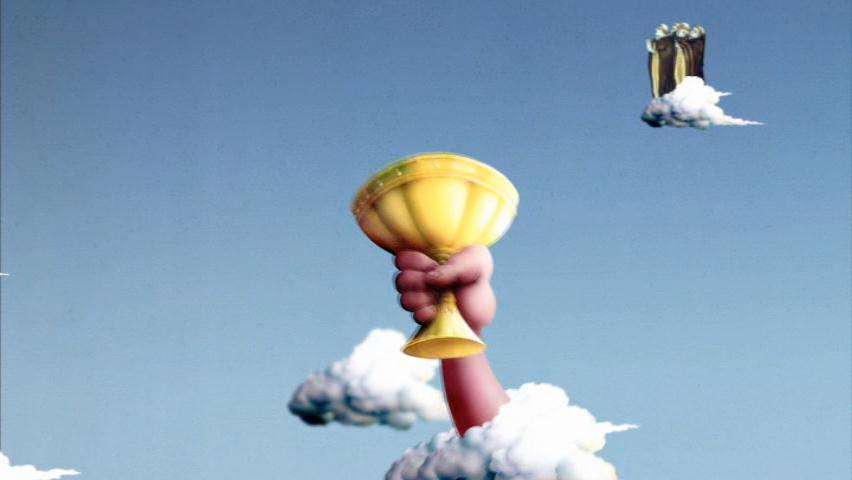
\includegraphics[width=0.8\textwidth]{grail.jpg}
  \caption[Voorbeeld figuur.]{\label{fig:grail}Voorbeeld van invoegen van een figuur. Zorg altijd voor een uitgebreid bijschrift dat de figuur volledig beschrijft zonder in de tekst te moeten gaan zoeken. Vergeet ook je bronvermelding niet!}
\end{figure}

\begin{listing}
  \begin{minted}{python}
    import pandas as pd
    import seaborn as sns

    penguins = sns.load_dataset('penguins')
    sns.relplot(data=penguins, x="flipper_length_mm", y="bill_length_mm", hue="species")
  \end{minted}
  \caption[Voorbeeld codefragment]{Voorbeeld van het invoegen van een codefragment.}
\end{listing}

\lipsum[7-20]

\begin{table}
  \centering
  \begin{tabular}{lcr}
    \toprule
    \textbf{Kolom 1} & \textbf{Kolom 2} & \textbf{Kolom 3} \\
    $\alpha$         & $\beta$          & $\gamma$         \\
    \midrule
    A                & 10.230           & a                \\
    B                & 45.678           & b                \\
    C                & 99.987           & c                \\
    \bottomrule
  \end{tabular}
  \caption[Voorbeeld tabel]{\label{tab:example}Voorbeeld van een tabel.}
\end{table}


%%=============================================================================
%% Methodologie
%%=============================================================================

\chapter{\IfLanguageName{dutch}{Methodologie}{Methodology}}%
\label{ch:methodologie}

%% TODO: In dit hoofstuk geef je een korte toelichting over hoe je te werk bent
%% gegaan. Verdeel je onderzoek in grote fasen, en licht in elke fase toe wat
%% de doelstelling was, welke deliverables daar uit gekomen zijn, en welke
%% onderzoeksmethoden je daarbij toegepast hebt. Verantwoord waarom je
%% op deze manier te werk gegaan bent.
%% 
%% Voorbeelden van zulke fasen zijn: literatuurstudie, opstellen van een
%% requirements-analyse, opstellen long-list (bij vergelijkende studie),
%% selectie van geschikte tools (bij vergelijkende studie, "short-list"),
%% opzetten testopstelling/PoC, uitvoeren testen en verzamelen
%% van resultaten, analyse van resultaten, ...
%%
%% !!!!! LET OP !!!!!
%%
%% Het is uitdrukkelijk NIET de bedoeling dat je het grootste deel van de corpus
%% van je bachelorproef in dit hoofstuk verwerkt! Dit hoofdstuk is eerder een
%% kort overzicht van je plan van aanpak.
%%
%% Maak voor elke fase (behalve het literatuuronderzoek) een NIEUW HOOFDSTUK aan
%% en geef het een gepaste titel.

\lipsum[21-25]



% Voeg hier je eigen hoofdstukken toe die de ``corpus'' van je bachelorproef
% vormen. De structuur en titels hangen af van je eigen onderzoek. Je kan bv.
% elke fase in je onderzoek in een apart hoofdstuk bespreken.

%\input{...}
%\input{...}
%...

%%=============================================================================
%% Conclusie
%%=============================================================================

\chapter{Conclusie}%
\label{ch:conclusie}

% TODO: Trek een duidelijke conclusie, in de vorm van een antwoord op de
% onderzoeksvra(a)g(en). Wat was jouw bijdrage aan het onderzoeksdomein en
% hoe biedt dit meerwaarde aan het vakgebied/doelgroep? 
% Reflecteer kritisch over het resultaat. In Engelse teksten wordt deze sectie
% ``Discussion'' genoemd. Had je deze uitkomst verwacht? Zijn er zaken die nog
% niet duidelijk zijn?
% Heeft het onderzoek geleid tot nieuwe vragen die uitnodigen tot verder 
%onderzoek?
\section{\IfLanguageName{dutch}{Resultaten}{Resultaten}}%
\label{sec:resultaten}
\subsection{\IfLanguageName{dutch}{Functionele vereisten}{Functionele vereisten}}%
\label{subsec:functionele vereisten}
\subsubsection{\IfLanguageName{dutch}{Monitoring}{Monitoring}}%
\label{subsubsec:monitoring}
De grootste use-cases van business zijn zeker behaald. Per lopende instantie van het simulatieproces is er een timeline met de huidige uitvoerder, de stappen en bereikte mijlpalen beschikbaar in sequentiële volgorde. Door deze informatie correct op te halen is het mogelijk om de klant in real-time te informeren van de status van zijn lopend proces in MyLiantis. Er zijn ook stappen gemaakt naar betere rapportage door de uitvoeringstijd per stap en eventuele afwijkingen in het normaal verloop zichtbaar te maken. Door dit af te nemen kan business intelligence opgezet worden om zo bottlenecks en anomalieën te detecteren op basis van servicelevel overeenkomsten. Het systeem weet ook hoeveel taken elke medewerker momenteel uitvoert en nog kan uitvoeren voor forecasting en balanceren van werklast. Dit is uiteraard relatief rudimentair, maar de technische haalbaarheid van het concept is zeker bewezen.
\subsubsection{\IfLanguageName{dutch}{Orkestratie}{Orkestratie}}%
\label{subsubsec:orkestratie}
In kader van orkestratie voldoet het systeem eveneens. Het genereert passende taken en zoekt de medewerker met het minst aantal actieve taken om deze uit te voeren tenzij expliciet aangewezen door de monitoring om dit niet te doen. In een latere iteratie kan dit verfijnd worden door bijvoorbeeld elke taak een granulair gewicht toe te kennen voor een betere balans. De API laat toe om alle huidige ingeplande taken voor een medewerker op te halen. Het is hierdoor mogelijk om een organische takenlijst voor te stellen in bijvoorbeeld de Digitale Cockpit. Verder kan het verloop van elke taak via de API doorgegeven worden opdat de data de werkelijkheid blijft volgen. Op de taak data kan eveneens rapportage gebouwd worden zodat bijvoorbeeld de doorlooptijd per type taak bepaald kan worden op data-gestuurde wijze.\newline
\subsection{\IfLanguageName{dutch}{Niet-functionele vereisten}{Niet-functionele vereisten}}%
\label{subsec:niet-functionele vereisten}
De proof-of-concept kan door zijn aard niet voldoen aan alle opgelegde functionele vereisten van het casusbedrijf gelet op het feit dat het geen toegang heeft tot de interne systemen. Het behalen van deze vereisten is een proof-of-concept dan ook geen must-have. De proof-of-concept voldoet echter wel aan volgende vereisten:
\begin{itemize}
  \item Het systeem is foutbestendig en gebouwd om zichzelf te remediëren na fouten.
  \item Het systeem voert alle synchrone bewerkingen uit aan 12 milliseconden of lager.
  \item Het kan een externe configuratie aanvaarden voor de mapping van de executie engine.
  \item De data is volledig generisch en bestaat louter uit referenties.
  \item Het systeem kan beveiligd worden via Spring Security.
  \item Het systeem genereert duidelijke logging bij elke handeling die aggregeerbaar is.
  \item Het systeem is volledig compliant met de interne technologie stack.
\end{itemize}

\subsection{\IfLanguageName{dutch}{Mogelijke verbeteringen}{Mogelijke verbeteringen}}%
\label{subsec:mogelijke verbeteringen}
Het project voldoet aan de vooropgestelde verwachtingen, maar elke systeem kan uiteraard iteratief verbeterd worden. Een eerste verbetering zou zijn om integraties bouwen met de masters rond processen en human resources. In de huidige opstelling is een singulier proces binnen scope, maar het zou elk proces moeten kunnen ondersteunen. Een integratie met een proces documentatietool zoals ARIS bij het casusbedrijf zou toelaten dat het systeem zijn executie engine dagelijks kan syncen.  Verder is de data van medewerkers en hun teams cruciaal om de juiste taken aan de juiste persoon te kunnen koppelen. \newline

Een tweede groot verbeterpunt is de inkomende monitoringdata uitbreiden en toegankelijker maken. Op basis van grondige analyse moet gekeken worden welke data het systeem zelf kan opvragen binnen de organisatie om de logs te verrijken en welke enkel het externe systeem kan leveren. Zodoende vergemakkelijkt de implementatie voor providers en verlaagt de load op hun systemen. Het beste scenario zou een plug-and-play library zijn die de providers implementeren en aanroepen om zo automatische de juiste data te formateren en door te sturen. \newline

Een derde groot verbeterpunt is het uitwerken van een extractie, transformatie en laadproces richting een datawarehouse. Het systeem zal naarmate meer processen toegevoegd worden aan de monitoring exponentieel meer data beginnen produceren die na ontsluiting van grote waarde is voor het bedrijf. Hoe sneller deze data kan landen bij de business intelligence experten, hoe hoger de business waarde van dit systeem zal zijn.

\section{\IfLanguageName{dutch}{Conclusies met betrekking tot Onderzoeksvraag}{Conclusies met betrekking tot onderzoeksvraag}}%
\label{sec:onderzoeksvraag conclusie}
\subsection{\IfLanguageName{dutch}{Probleemstelling}{Probleemstelling}}%
\label{subsec:probleemstelling conclusie}
De centrale probleemstelling uit hoofdstuk~\ref{sec:probleemstelling} van dit onderzoek heeft een heel duidelijk antwoord gekregen. Door de literatuurstudie en analyse heen werd kritisch gezocht naar de vereisten en architectuur die nodig is om custom proces monitoring en orkestratie te implementeren binnen een bedrijf met veel custom development toepassingen. Hiervoor werd eerst een theoretisch en dan een praktisch antwoord geformuleerd op basis van de noden van het casusbedrijf.

\subsection{\IfLanguageName{dutch}{Probleemdomein}{Probleemdomein}}%
\label{subsec:probleemdomein conclusie}
De antwoorden voor de vragen uit het probleemdomein in hoofdstuk~\ref{sec:probleemdomein} worden hier expliciet opgelijst:
\begin{itemize}
  \item Op basis literatuur uit het werkveld werden de theoretische functionele in hoofdstuk~\ref{sec:proces monitoring} en niet-functionele vereisten in hoofdstuk~\ref{sec:proces orkestratie} gevonden.
  \item In hoofdstuk~\ref{sec:proces monitoring en orkestratie als IT-systeem} werd gekeken naar de opbouw en mogelijkheden van zowel monolithisch out-of-the-box systemen als gedistribueerde systemen van eigen makelij.
  \item Op basis van workshops in hoofdstuk~\ref{sec:functionele vereisten} met business stakeholders en een brainstorming met een systeem architect in hoofdstuk~\ref{sec:niet-functionele vereisten} werden de praktische functionele en niet-functionele vereisten die specifiek gelden voor een HR-bedrijf gevonden.
  \item Op basis van een brainstorming met een systeem architect in hoofdstuk~\ref{subsec:brainstorming sessie met systeem architect} werden de technisch en architecturale uitdagingen in kaart gebracht voor een bedrijfsomgeving met veel custom development
\end{itemize}

\subsection{\IfLanguageName{dutch}{Oplossingsdomein}{Oplossingsdomein}}%
\label{subsec:oplossingsdomein conclusie}
De antwoorden voor de vragen uit het oplossingsdomein in hoofdstuk~\ref{sec:oplossingsdomein} worden hier expliciet opgelijst:
\begin{itemize}
  \item Bij het opmaken van het design van het systeem in hoofdstuk~\ref{sec:design} werd gevonden hoe dergelijke systemen in een bedrijfsomgeving met veel custom development geïmplementeerd worden. 
  \item Bij de validatie in hoofdstuk~\ref{sec:validatie} en de visualisatie in hoofdstuk~\ref{sec:visualisatie} werden de criteria gevonden tijdens de analyse in hoofdstuk~\ref{ch:analyse} getoetst om te ontdekken aan welke criteria dergelijke systemen moeten voldoen om succesvolle proces monitoring en orkestratie te bereiken binnen het casusbedrijf.
\end{itemize}

Het is hierbij duidelijk dat er in het werkveld plaats is voor dergelijk systeem. Een omgeving met veel custom development en legacy vereist eveneens een monitoring en orkestratie systeem van eigen makelij die kan voldoen aan de specifieke eisen van het bedrijf. Out-of-the-box systemen zijn ook zeker bruikbaar, maar bieden in deze context onvoldoende antwoord op deze eisen zonder dure integraties en aanpassingen van legacy systemen. Er zal echter altijd een afweging blijven tussen kosten en baten in de build versus buy discussie die voor elk bedrijf een antwoord zal genereren.

\section{\IfLanguageName{dutch}{Algemene Conclusie}{Algemene Conclusie}}%
\label{sec:algemene conclusie}
In dit werk werd onderzocht welk de vereisten zijn waaraan een systeem moet voldoen en welke software architectuur gepast is om custom proces monitoring en orkestratie te implementeren binnen een bedrijf met veel custom development applicaties. \newline

Allereerst werd een literatuurstudie gedaan om te begrijpen hoe hedendaagse systemen binnen het werkveld werken, wat hun mogelijkheden zijn en wat de best practices zijn bij het ontwerpen van dergelijk systeem. Op basis van een analyse binnen casusbedrijf Liantis die voldoet aan bovenstaande criteria werden hun vereisten omgezet in een lijst van functionele en niet-functionele vereisten die representatief zijn voor het bedrijf zelf als andere bedrijven van een gelijkaardig profiel.\newline

Verder werd een design gemaakt die architecturaal en functioneel voldoet aan de eisen van het casusbedrijf waarbij zowel proces- als systeem-agnostisch werd gewerkt om zo tegemoet te komen aan de technische en architecturale uitdagingen waar het bedrijf mee kampt door zijn veelvoud aan custom development.\newline

Dit design werd dan omgezet in een werkende proof-of-concept die gesimuleerde data van een proces kon verwerken in geconsolideerde executie logs die afnemers via een duidelijke API kunnen gebruiken om vereiste use-cases gevonden tijdens de analyse op te leveren.  Op basis van de data kon dit systeem ook taken aanmaken en toekennen aan medewerkers binnen het bedrijf. Op basis van een duidelijke API konden afnemers hiermee een taakoverzicht bouwen voor de betrokkenen medewerkers en die status van deze taken correct aanpassen op basis van hun verloop. Een rudimentaire versie van de realisaties die het casusbedrijf wil bouwen werd ook opgeleverd.\newline

Het resultaat toont daarmee hoe dergelijk systeem succesvol geïmplementeerd kan worden in een bedrijfsomgeving met veel custom development en vormt zo een blauwdruk waarmee een succesvolle proces monitoring en orkestratie bereikt kan worden dat reproduceerbaar is binnen soortgelijke bedrijven in het werkveld.\newline

Het doel van dit onderzoekswerk is daarmee bereikt waardoor de weg nu vrij is om dit systeem te implementeren bij het casusbedrijf. Hiervoor zijn er al reeds concrete stappen uitgevoerd dit kwartaal met uitzicht op verdere iteratieve uitbreiding in volgende kwartalen op basis van de reeks bereikte resultaten. Hiermee is het bijkomend doel van dit werk succesvol behaald en zal het werk uitgevoerd in kader van deze bachelor proef nog verder vervolgd worden in professionele setting.




%---------- Bijlagen -----------------------------------------------------------

\appendix

\chapter{Onderzoeksvoorstel}

Het onderwerp van deze bachelorproef is gebaseerd op een onderzoeksvoorstel dat vooraf werd beoordeeld door de promotor. Dat voorstel is opgenomen in deze bijlage.

%% TODO: 
%\section*{Samenvatting}

% Kopieer en plak hier de samenvatting (abstract) van je onderzoeksvoorstel.

% Verwijzing naar het bestand met de inhoud van het onderzoeksvoorstel
%---------- Inleiding ---------------------------------------------------------

\section{Inleiding}%
\label{sec:inleiding}

\subsection{Context en Onderzoeksvraag}

Dit werk richt zich op het verbeteren van process governance door middel van process monitoring en orchestration, specifiek binnen het bedrijf Liantis, een grote Belgische onderneming actief in de HR sector. Liantis biedt oplossingen in kader van payroll, preventie/welzijn op het werk en ondersteuning aan zelfstandigen. Omdat het bedrijf een wildgroei aan processen heeft die steeds complexer en dynamischer worden, heeft het Liantis moeite om een consistent en betrouwbaar beheer van zijn processen te waarborgen. Vooral door beperkte mogelijkheden om real-time inzicht te krijgen in de prestaties van hun medewerkers, ontstaan er regelmatig inefficiënties en compliance-uitdagingen. Voor business-managers en -analisten binnen dit bedrijf vormt dit een knelpunt bij het waarborgen van de procesbetrouwbaarheid en het naleven van interne en externe regelgeving. De centrale onderzoeksvraag luidt dan ook "Hoe kan process monitoring en orchestration bijdragen aan een effectieve ondersteuning van process governance?" en dit praktisch toegepast binnen het specifieke geval van Liantis. Een bijkomende vraag is "Wat zijn de technische uitdagingen bij de implementatie van process monitoring en orchestration systemen bij Belgische bedrijf met zowel inhouse als externe software?" omdat deze natuurlijk zal voortvloeien vanuit de casus Liantis.

\subsection{Doel en Resultaat}

Het doel van deze bachelorproef is om een concreet raamwerk en aanbevelingen te ontwikkelen voor het implementeren van process monitoring en orchestration om zo de process governance binnen Liantis te optimaliseren. Verder zal het een proof-of-concept realizeren waarbij we dit toepassen op een specifiek gekozen process. Dit zal dan gebruikt worden om de relevante stakeholders te overtuigen om dit verder uit te rollen naar andere processen.  Hiervoor zal eerst een uitgebreide literatuurstudie worden uitgevoerd om inzicht te krijgen in bestaande methoden en tools op het gebied van process monitoring en orchestration. Vervolgens wordt er een casestudie uitgevoerd binnen het bedrijf om de huidige knelpunten in kaart te brengen en de impact van mogelijke oplossingen te evalueren. Op basis hiervan zal een proof-of-concept ontwikkeld worden waarbij we aantonen hoe dit praktisch een specifiek gekozen complex bedrijfsprocess zal ondersteunen. Het beoogde eindresultaat voor een succesvolle bachelorproef bestaat uit een gedetailleerd implementatieplan dat de IT-afdeling van Liantis helpt om monitoring en orchestration op een effectieve manier in de governance-structuur te integreren met een proof-of-concept die kan dienen als sjabloon voor verdere implementatie. 

%---------- Stand van zaken ---------------------------------------------------

\section{Stand Van Zaken}%
\label{sec:stand_van_zaken}
\subsection{Business Process Management en Governance}

Het domein van business process management (BPM) en governance richt zich op het verbeteren van bedrijfsprocessen door middel van monitoring, analyse, en optimalisatie. BPM biedt organisaties de mogelijkheid om processen te stroomlijnen en deze af te stemmen op de strategische doelen van de organisatie \autocite{Dumas2018}. Binnen deze context spelen process monitoring en orchestration een cruciale rol. Deze technologieën maken het mogelijk om bedrijfsprocessen op een efficiënte en geautomatiseerde manier te beheren en aan te passen \autocite{Weske2019}.

\subsection{Monitoring, Mining en Orchestration}

Process monitoring is essentieel binnen BPM omdat het organisaties near-realtime inzicht geeft in de prestaties van hun bedrijfsprocessen, waardoor afwijkingen of inefficiënties snel kunnen worden geïdentificeerd \autocite{Janiesch2012}. Dit is dan voedingsbodem voor process mining, waarbij we de logs uit de monitoring gebruiken om tot analytische inzichten te komen. Process mining biedt niet alleen inzicht in het huidige verloop van processen maar maakt ook een data-gedreven optimalisatie mogelijk door onregelmatigheden bloot te leggen die vaak onzichtbaar blijven bij traditionele monitoring \autocite{Aalst2016}. Daarnaast kan Business Activity Monitoring (BAM) organisaties helpen om niet alleen retrospectief maar ook proactief op afwijkingen te reageren, wat waardevol is voor processen met hoge compliance-eisen \autocite{Janiesch2012}. Process orchestration gaat een stap verder dan monitoring door bedrijfsprocessen te automatiseren en te coördineren op basis van vastgelegde beleidslijnen en workflows. Dit is vooral nuttig voor organisaties die streven naar consistentie en compliance in hun bedrijfsvoering \autocite{Weske2019}. 

\subsection{Open Vragen}

De grote open vraag die heeft geleid tot dit onderzoek is de technische uitdaging van het implementeren van deze systemen binnen een groot bedrijf zoals Liantis. Net zoals veel bedrijven is Liantis immers organisch gegroeid en bevat het niet enkel veel inhouse legacy systemen, maar ook aangekochte systemen. Dergelijke monitoring en orchestratie systemen moeten op een agnostische manier kunnen omgaan met de output van allerhande processen en systemen. De implementatie van deze systemen in een bedrijfscontext brengt dus verschillende technische uitdagingen met zich mee die vaak custom oplossingen vereisen. Vakliteratuur geeft een aantal interessante opties zoals het gebruik van middleware \autocite{Weber2018}, maar er is een zeer duidelijke lacune te zien binnen het domein om te onderzoeken. 

\subsection{Vergelijkbare Studies en Unieke Waarde}

De waarde van dit domein is al zeker en vast bewezen door Vergelijkbare studies binnen grote organisaties \autocite{Harmon2014} die benadrukken dat de implementatie van geavanceerde monitoring- en orchestrationtechnieken helpen om consistent aan governance- en compliance-vereisten te voldoen. Dit onderzoek biedt echter een unieke bijdrage door zich te richten op de praktische toepasbaarheid van deze technieken bij een groot Belgische bedrijf wiens IT-context breed toepasbaar is. Door dit uit te werken zal er een praktisch raamwerk bestaan voor de implementatie van dergelijke systemen binnen een bedrijf met dergelijk profiel met proof-of-concept dat kan dienen als bluedruk voor veel Belgische bedrijven. 

%---------- Methodologie ------------------------------------------------------
\section{Methodologie}%
\label{sec:methodologie}

Om de onderzoeksvraag te beantwoorden en een effectieve aanpak te ontwikkelen voor de implementatie van process monitoring en orchestration binnen Liantis, wordt gebruikgemaakt van een gefaseerde onderzoeksmethodologie die literatuurstudie, case study-analyse, requirements-analyse en een proof-of-concept ontwikkeling omvat. Deze combinatie van technieken waarborgt zowel theoretische onderbouwing als technische diepgang, wat essentieel is voor het creëren van een valide en werkbaar implementatiemodel.

\subsection{Fase 1: Literatuurstudie (2 weken)}

De eerste fase bestaat uit een gedetailleerde literatuurstudie. Hierbij worden academische artikelen en technische bronnen over business process management, monitoring, orchestration, en implementatie-uitdagingen grondig geanalyseerd. Deze studie heeft als doel om een diepgaand inzicht te verkrijgen in de huidige stand van zaken en de typische uitdagingen en succesfactoren binnen BPM-implementaties voor process governance. De bevindingen uit de literatuurstudie vormen de theoretische basis van het onderzoek en dienen als referentiekader voor de verdere fasen. \\

\textbf{Deliverable:} een theoretisch component met gedocumenteerde inzichten over BPM-standaarden, technische obstakels, en oplossingen voor de organisatie.

\subsection{Fase 2: Requirements-analyse binnen Liantis (2 weken)}

Om de specifieke behoeften en uitdagingen van de casusorganisatie vast te stellen, wordt een requirements-analyse uitgevoerd door middel van gestructureerde workshops met stakeholders binnen de organisatie, zoals IT-managers, procesanalisten, en compliance-officers. Verder wordt de bestaande IT-infrastructuur bekeken om te kijken hoe we dit het beste inpassen om de impact minimaal te houden. We bepalen hier ook het complexe process dat in scope zal zijn voor onze proof-of-concept. \\

\textbf{Deliverable:} een requirementsrapport met gedetailleerde, gevalideerde vereisten voor de implementatie.

\subsection{Fase 3: Technische en Functionele Analyse (2 weken)}

Na de requirements-analyse wordt een technische analyse uitgevoerd om geschikte tools en technologieën te selecteren. Hierbij zoeken we naar een process documentatie tool waarmee we kunnen integreren als bron van waarheid, modeleren we een architectuur voor deze systemen, schrijven we een contract uit dat alle systemen gaan gebruiken voor de monitoring en orchestratie en voeren we de analyse uit voor de proof-of-concept.  \\

\textbf{Deliverable:} design documenten voor de process monitoring en orchestration tools met implementatieplan.

\subsection{Fase 4: Proof-of-Concept Ontwikkeling en Validatie (1 maand)}

In deze fase wordt een proof-of-concept ontwikkeld om de haalbaarheid van het voorgestelde implementatiemodel te testen. De PoC omvat de integratie van de monitoring- en orchestration systeem met een voorbeeldproces van de Liantis. Dit proces wordt gesimuleerd met representatieve data om de configuratie van monitoring en event-triggered orchestration te testen. Deze proof-of-concept zal dan gebruikt worden stakeholders te overtuigen en als blauwdruk voor verdere processen. \\

\textbf{Deliverable:} een gedetailleerd PoC-rapport en werkend prototype dat het systeem demonstreert.

%---------- Verwachte resultaten ----------------------------------------------
\section{Verwachtingen}%
\label{sec:verwachtingen}
De verwachting binnen dit onderzoek is dat er een implementatieplan zal ontstaan die toelaat om process governance te waarborgen binnen Liantis door te steunen op een sterk framework van monitoring en orchestration met een proof-of-concept om stakeholders te overtuigen. Dit zal dan fungeren als verdere impetus voor het uitwerken van dit systeem binnen de organisatie met als gevolg consistentere processen die makkelijker geoptimaliseerd kunnen worden.

Verder is het mijn verwachting dat de resultaten uit dit onderzoek toepasbaar zullen zijn op bedrijven die een gelijkaardig profiel hebben als Liantis. Liantis is binnen zijn IT-context zeker geen uitzondering en het is mijn doel om binnen dit onderzoek Liantis als case study te gebruiken om zo een framework te ontwikkelen waarmee veel meer bedrijven gediend zijn.



%%---------- Andere bijlagen --------------------------------------------------
% TODO: Voeg hier eventuele andere bijlagen toe. Bv. als je deze BP voor de
% tweede keer indient, een overzicht van de verbeteringen t.o.v. het origineel.
%\input{...}

%%---------- Backmatter, referentielijst ---------------------------------------

\backmatter{}

\setlength\bibitemsep{2pt} %% Add Some space between the bibliograpy entries
\printbibliography[heading=bibintoc]

\end{document}
